\chapter{Herramienta de generación de árboles de comportamiento}
\label{cap:descripcionTrabajo}

% \begin{quote}
%     \chapterquote{In the distant future.\\
%         In a land abandoned by man.\\
%         Machines wage a continuous war.\\
%         Unaware of the futility of their actions.}{Nier Automata}
% \end{quote}

% \input{Capitulos/DescripcionTrabajo/Traje}
% \input{Capitulos/DescripcionTrabajo/BusquedaDataset}
% \input{Capitulos/DescripcionTrabajo/DatasetArtificial}
% \input{Capitulos/DescripcionTrabajo/DatasetReal}
% \input{Capitulos/DescripcionTrabajo/Modelos}
% \input{Capitulos/DescripcionTrabajo/AplicacionFinal}

Debido al proceso tedioso y costoso en tiempo de formación y producción que conlleva a los diseñadores la creación de árboles de comportamiento (BTs) de forma constante para idear a los diferentes personajes no jugador (NPCs), el objetivo general de este trabajo es la creación de una herramienta que sea capaz de generar BTs funcionales que sirvan de base para rebajar la carga de trabajo de los diseñadores.
Para ello se busca un modelo que sea completamente opaco al usuario, que dé resultados en un tiempo inferior a la alternativa ya existente con una calidad similar y que sea sencilla de usar sin requerir muchos conocimientos técnicos para, además, ayudar a diseñadores con un perfil no tan técnico a desarrollar con mayor facilidad.

Con esta idea en mente y gracias a los avances que se han producido en el campo de los modelos del lenguaje, se ha desarrollado un modelo de herramienta basada en generación mediante LLMs, ya que ofrece la ventaja de que los usuarios puedan explicar el comportamiento deseado en lenguaje natural.
Como esta herramienta debería ser de fácil uso para los diseñadores y programadores, se propone un modelo en el que, sin salir de un proyecto de Unreal Engine, se puedan generar los BTs mediante su propia interfaz.

\section{Diseño del pipeline del modelo propuesto de generación de árboles de comportamiento}
\label{sec:ModeloBT}

Antes de diseñar e implementar la herramienta se ha buscado tener claro el diseño de cuál debería ser el flujo de ejecución, así como los diferentes módulos que la iban a componer.

\begin{figure}[H]
    \centering
    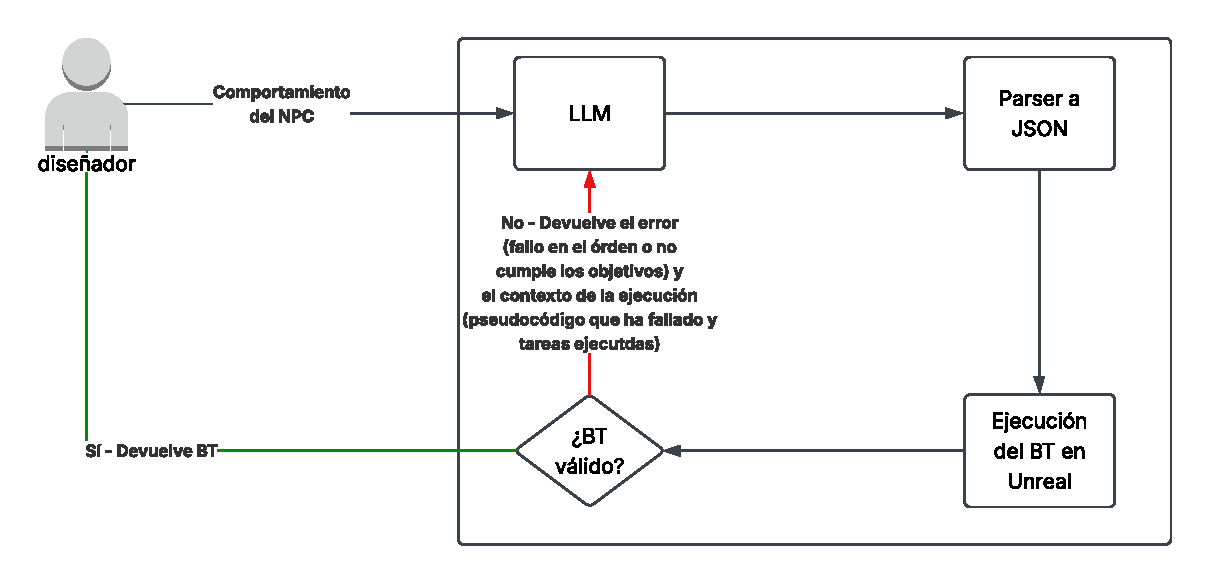
\includegraphics[width=1.0\textwidth]{Imagenes/Vectorial/DiagramaHerramienta.pdf}
    \caption[Diagrama de la herramienta propuesta]{Diagrama donde se visualiza el flujo de la herramienta propuesta.}
    \label{fig:diagramaHerramienta}
\end{figure}

En la figura \ref{fig:diagramaHerramienta} se puede ver el flujo de ejecución propuesto:

\begin{enumerate}
    \item El diseñador describe el comportamiento buscado para un NPC.
    \item Fuera del entorno del motor de videojuegos se genera el árbol de comportamiento mediante LLMs en un formato JSON.
    \item El motor de videojuegos traduce y crea el árbol de comportamiento generado.
    \item Se ejecuta el árbol.
    \item Opcionalmente se valida el árbol de forma automática. En caso de ser un árbol válido se termina la ejecución. En caso contrario se devuelve al modelo generador el árbol fallido y se le avisa del error.
\end{enumerate}

Este pipeline busca la independencia entre el motor de videojuegos y los modelos LLM, así como una opacidad de la generación frente a los usuarios y la simplicidad para diseñadores que no tengan un perfil muy técnico.

En las siguientes secciones de este capítulo se explicará el entorno de pruebas desarrollado para este trabajo, así como la implementación de la generación de los BTs, la validación de éstos y las pruebas a usuarios realizadas.
\section{Descripción del entorno}
\label{sec:DescripcionEntorno}

Para poder desarrollar la herramienta se han creado unos entornos de pruebas basado en Unreal Engine 5.7.
Son estos entornos los que se van a comunicar con el agente \gls{LLM} de Python.

Estos entornos, de los que se pueden ver un ejemplo en la figura \ref{fig:entorno}, constan de un agente (el \gls{npc} que va a seguir el comportamiento buscado) cuyo controlador es una clase que hereda de la clase de Unreal Engine ``AIController''.
Esta clase contiene los componentes de \gls{BB} y \gls{BT} necesarios para la futura ejecución de un \gls{BT}.
En la misma figura se puede apreciar la interfaz en la que el usuario debe introducir la información necesaria para la generación del \gls{BT}: la descripción del comportamiento buscado, el nombre con el que se va a guardar el \gls{BT} generado, las entradas de la \gls{BB}, el agente que va a ejecutar el \gls{BT} generado y, opcionalmente, el nombre del archivo de validación del \gls{BT} generado.
Esta información la debe contener un actor, llamado en la captura ``BTGeneratorManager'', que tenga un componente llamado ``BTGenerator''.
Este componente de actor es el encargado de lanzar el proceso de Python con la información que el usuario haya puesto, y el que comienza la ejecución de las pruebas del \gls{BT} generado.
Para comenzar la ejecución se debe pulsar el botó ``GenerateBT'' que se aprecia en la captura.

\begin{figure}[H]
    \centering
    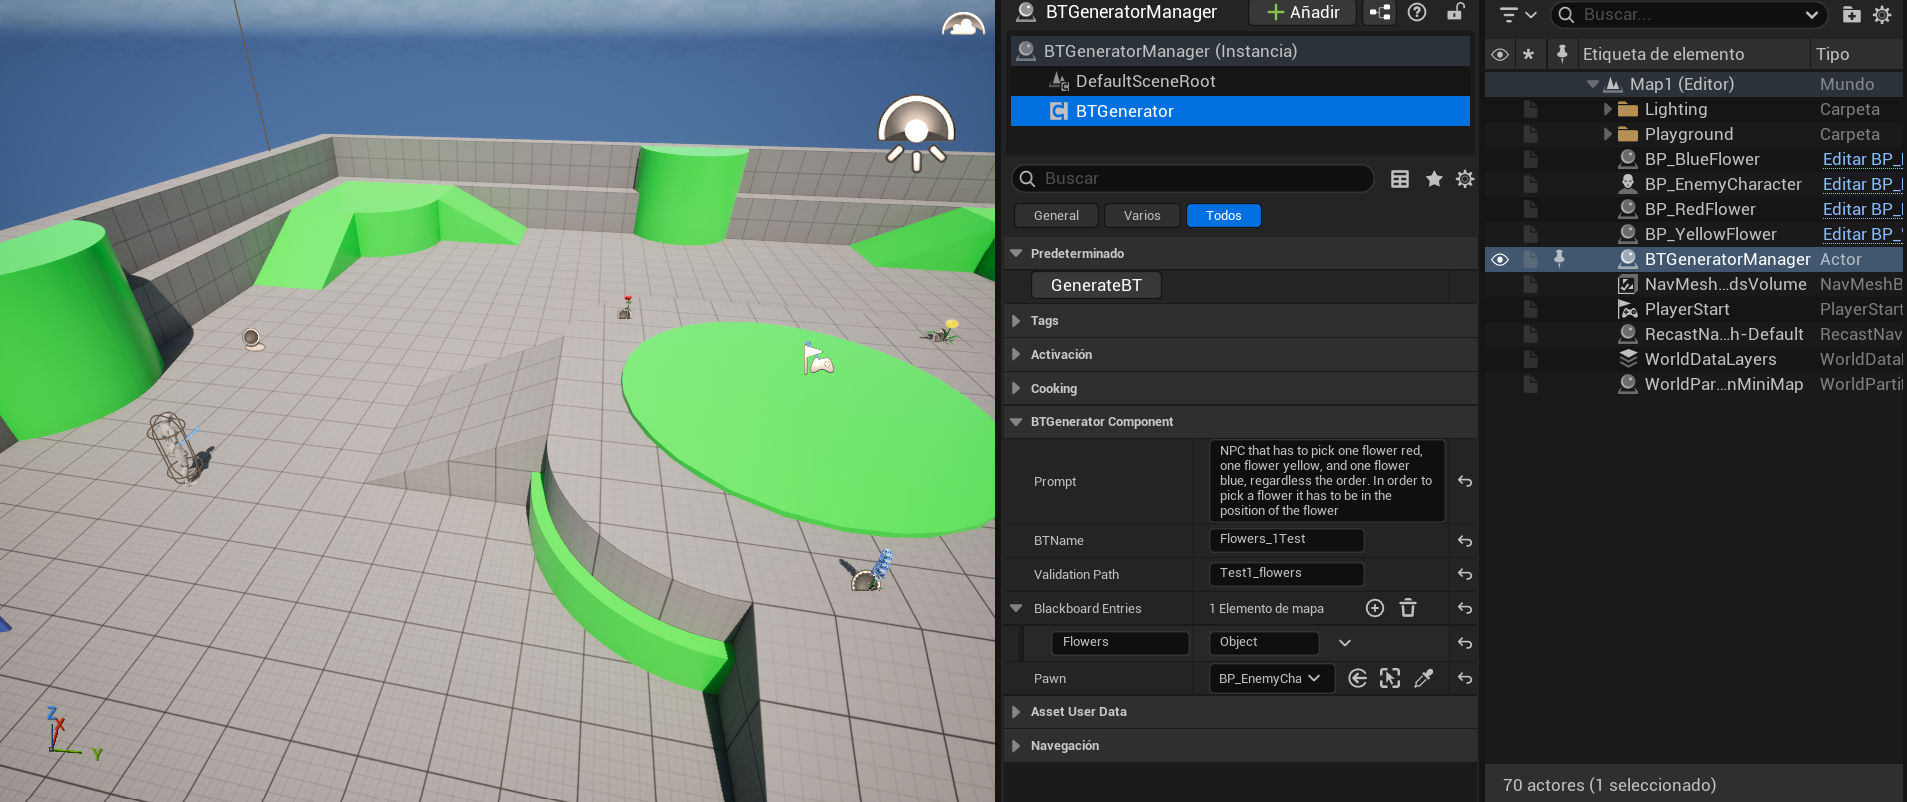
\includegraphics[width=1.0\textwidth]{Imagenes/Bitmap/Entorno1.png}
    \caption[Entorno de desarrollo]{Captura de pantalla de uno de los entornos creados para el desarrollo de la herramienta.}
    \label{fig:entorno}
\end{figure}

Junto con este agente se han preparado una serie de tareas (los cuales servirán como nodos terminales de los árboles) y condicionales que sirven como base para poder crear unos comportamientos de prueba.
Estas tareas y condicionales son introducidos en una clase ``BTFactory'', la cual es un \gls{Abstract Factory} implementado para la construcción de los \glspl{BT}.
Esta clase, la cual se inicializa desde el componente ``BTGeneratorComponent'', contiene tres diccionarios que guardan las tareas, las tareas que necesitan una variable de la \gls{BB} y los condicionales.
Estos diccionarios reciben como clave un string, que es la ID de la tarea o el condicional, y como valor una función (implementada en la propia clase) que crea el objeto que se ha pedido.
Además esta clase tiene otro diccionario que contiene la descripción de cada tarea y condicional, la cual es fundamental para la futura generación de los \glspl{BT}.
Para registrar una nueva clase en esta factoría se debe llamar a las funciones ``RegisterTask'', ``RegisterBlackboardTask'' o ``RegisterDecorator'', las cuales son funciones template en las que se les debe poner la clase que se desea ser introducida y pasar como argumentos el ID que se desee poner y la descripción de lo que realiza la tarea o lo que revisa el condicional.
Además, para las clases que requieran una variable de la \gls{BB} es recomendable introducir qué tipo de variable se requiere.

Las tareas, junto con sus descripciones en español (en el trabajo realizado las descripciones han sido escritas en inglés para respetar el idioma del prompt) que se han creado para estas pruebas son las siguientes:

\begin{itemize}
  \item \texttt{RotateToFaceBBEntry}: Rotar hasta encarar objetivo. El objetivo tiene que ser de tipo ``Objeto''.
  \item \texttt{ChasePlayer}: Perseguir al jugador.
  \item \texttt{MoveTo}: Mover a la posición u objeto de destino. La variable objetivo tiene que ser de tipo ``Objeto'' o ``Vector3''
  \item \texttt{FindRandomPatrol}: Elegir un punto aleatorio del mapa y guardarlo como objetivo.
  \item \texttt{Wait}: No hacer nada.
  \item \texttt{PickRedFlower}: Coger una flor roja.
  \item \texttt{PickBlueFlower}: Coger una flor azul.
  \item \texttt{PickYellowFlower}: Coger una flor amarilla.
  \item \texttt{PickBlackFlower}: Coger una flor negra.
  \item \texttt{ChooseRedFlower}: Elegir una flor roja como objetivo.
  \item \texttt{ChooseBlueFlower}: Elegir una flor azul como objetivo.
  \item \texttt{ChooseYellowFlower}: Elegir una flor amarilla como objetivo.
  \item \texttt{ChooseBlackFlower}: Elegir una flor negra como objetivo.
  \item \texttt{Attack}: Atacar si hay algún objetivo cerca.
  \item \texttt{SelectWaypoint}: Elegir un punto de ruta aleatorio y establecerlo como objetivo. El objetivo debe ser de tipo ``Objeto''
\end{itemize}

Los condicionales implementados, junto con sus descripciones en español (al igual que las tareas, las descripciones en el trabajo están en inglés), son los siguientes:

\begin{itemize}
  \item \texttt{HasLineOfSight?}: Cierto si el jugador está en línea de visión, falso si no. La variable que verifica tiene que ser de tipo ``Bool''
  \item \texttt{IsItNear?}: Cierto si la distancia entre el ejecutor y el jugador es menor o igual que un umbral prefijado, falso en caso contrario. El objetivo tiene que ser de tipo ``Objeto''.
\end{itemize}

Las tareas y condicionales que necesiten una variable de la \gls{BB} necesitan seleccionarla desde el objeto de la \gls{BB} (llamado en Unreal ``BlackboardData'') a través de una variable que tienen los condicionales y las tareas que hereden de la clase de Unreal ``BTTask\_BlackboardBase'', que son las tareas que requieren de una variable.
Sin embargo esta variable es protegida, por lo que se ha creado una interfaz intermedia llamada ``BaseTask'' (de la que heredan todas las tareas que requieran una variable) que contiene las funciones necesarias para acceder a esta variable protegida que permite seleccionar la variable deseada de la \gls{BB}.

El número de terminales y decoradores disponibles en esta implementación es reducido, pero sirve
como sistema de prueba para la generación y la propuesta de evaluación.

Para la generación del JSON se ha seguido una definición de JSON Schema (Draft 2020-12) que delimita la estructura de la generación del JSON para adaptarlo a las necesidades del trabajo.
Este JSON Schema consta de dos partes: el \gls{BB} y el \gls{BT}.
El \gls{BB} es una lista de objetos JSON que contienen solo un par clave-valor, donde la clave es el nombre de la variable y el valor es el tipo de la variable (Bool, Int, Float, Vector, Object o String).
El \gls{BT} consta de un nodo (la raíz) que debe contener el tipo de nodo (Task, Sequence, Selector o Parallel), una lista de decoradores (en el caso de no tener se debe quedar vacía), la cual consiste en objetos JSON que debe contener como clave el nombre del decorador y como valor la varaible de la \gls{BB} que va a usar, y una lista de nodos hijos.
Estos nodos hijos siguen la misma estructura que la raíz.
Como propiedades adicionales, puede contener una lista de nombres de variables de la \gls{BB} que vaya a necesitar, y, en el caso de ser una tarea, debe tener el ID de ésta.
Este esquema se puede encontrar en el apéndice \ref{appendix:Schema}

Para cuando el modelo haya generado el JSON con el \gls{BT}, la clase ``BTGeneratorComponent'' entra en el modo de juego.
Es en este momento donde el \gls{npc}, desde su función ``BeginPlay'' (función de Unreal que es llamada cuando se inicia el juego), coge el nombre del archivo JSON generado para traducirlo a la lógica de Unreal.
Esta traducción la hace la clase ``BTConstructor'', la cual es una clase que sigue el patrón \gls{Singleton} que es inicializada desde la clase ``BTGeneratorComponent''.
Para la traducción se le pasa a la clase el nombre del archivo y el componente de \gls{BB} que debe contener el \gls{npc} mediante el método ``CreateBT''.
Este método crea un \gls{BT} (clase ``BehaviorTree'') y un \gls{BB} (clase ``BlackboardData'') que serán rellenados con la información del JSON.

Lo primero que se traduce es el \gls{BB} gracias al método ``CreateBlackboardAsset'', el cual recorre toda la lista de vaiables para, dependiendo del tipo de ésta, crear un nuevo objeto de Unreal de tipo ``BlackboardkeyType\_XX'' (donde las XX es el tipo de la variable).
Éstas se guardan dentro del campo ``KeyType'' de una variable creada de tipo ``BlackboardEntry'', que será agregada al campo ``Keys'' de la variable de tipo ``BlackboardData''.
Cuando ya se han creado todas las variables de la \gls{BB} se inicializa mediante el método ``InitializeBlackboard'' del componente ``BlackboardComponent''.

Finalmente se crea el \gls{BT} mediante el método recursivo ``CreateNode''.
Inicialmente crea un objeto de tipo ``FBTCompositeChild'' en el que se guardará y devolverá el nodo que se le haya pasado como parámetro (inicialmente el nodo raíz).
Si no es de tipo ``Task'' se crea un objeto de tipo ``BTCompositeNode'', del cual heredan los nodos compuestos (Selector, Sequence y Parallel) para, posteriormente y de forma recursiva, incializar los nodos hijos comprendidos dentro de la lista ``Nodes'' y establecérselos como sus hijos.
Si por el contrario es de tipo ``Task'' se le pide a la clase ``BTFactory'' una nueva instancia de esa tarea (si no existe esta tarea se devuelve un nodo vacío).
Además, si necesita alguna variable de la \gls{BB}, se llama a las funciones necesarias de éstas tareas para establecérsela.
Finalmente, tanto como para las tareas como para los nodos compuestos, se recorren sus decoradores para inicializarse de la misma forma que las tareas: pidiéndole a ``BTFactory'' una instancia de esa clase y estableciendo las variables de la \gls{BB} necesarias.
\section{Generación de los \glspl{BT}}
\label{sec:GeneracionBTs}

% Una vez se lanza el proceso de Python, se recogen los argumentos de la ejecución mediante el módulo ``sys''.
En un principio se planteó la generación de los \glspl{BT} de forma directa, en la que se le pasaba el prompt del usuario a un modelo local y éste generaba un \gls{BT} en el formato JSON especificado en el apéndice \ref{appendix:Schema}.
Este planteamiento se realizaba mediante el módulo de Python ``guidance'', el cual permite forzar un formato de salida a un modelo de \gls{Ollama}.
Para este caso se probaron diferentes modelos, todos probados bajo el mismo escenario y con la temperatura en 0.0:
\begin{itemize}
    \item \texttt{Prompt}: \gls{npc} that, constantly, select a random point from the map, goes to the point and waits a time.
    \item \texttt{Acciones disponibles}: ChooseRandomPoint, MoveTo, WaitTime, RotateToFaceBBEntry.
    \item \texttt{Variables de la \gls{BB}}: Point (Vector3)
\end{itemize}

Se buscó una tarea sencilla para establecer un baseline de los modelos.
Los modelos probados para este planteamiento, con sus parámetros, su tiempo de ejecución y su resultado se pueden ver en la tabla \ref{tab:modelos-guidance}:

\begin{longtblr}[
    caption = {Modelos probados para la generación directa del JSON mediante guidance.},
    label = {tab:modelos-guidance}
]{
colspec={|l|l|l|},
rowhead=1,
hlines,
row{even}={gray9},
cells   = {font=\footnotesize\linespread{0.84}\selectfont},
}
    \hline
    Modelo    & Parámetros  & Tiempo de ejecución\\ \hline
    microsoft/Phi-4-mini-instruct    & 4B   & ~10 segundos \\
    qwen2.5:7b    & 7B  & ~20 segundos \\
    Qwen/Qwen2.5-Coder-7B-Instruct  & 7B    & ~30 minutos \\
    llama3.1:8b  & 8B   & ~2 horas  \\
    deepsek-r1:8b & 8B  & >2 horas \\ \hline
\end{longtblr}

Los modelos de menor tamaño no generaban buenos \glspl{BT} para una tarea tan sencilla (como tareas que faltaban o variables de la \gls{BB} mal asignadas).
Sin embargo, los modelos grandes si conseguían generar \glspl{BT} que cumplían con la función que se les pedía, aunque añadiendo más tareas de las necesarias.
Pero, como se puede observar en la tabla, para conseguir esos \glspl{BT} la ejecución podía tardar horas, por lo que también debían ser descartados.
Tanto la malfuncionalidad de los modelos pequeños como la tardanza de los modelos grandes se puede explicar por el funcionamiento de guidance y la complejidad recursiva del JSON Schema empleado, por lo que esta primera generación debería ser descartada.

En base a otros trabajos relacionados como \cite{ZKTP} o \cite{ReAcTree} se replanteó la generación para dividirlo en subtareas con el fin de simplificar la tarea al \gls{LLM}.
Para ello se encargaban cuatro agentes \gls{LLM}, cada uno con un rol distinto.
El primero se encargaba de dividir la acción mandada por el usuario mediante el prompt en subtareas.
En el ejemplo de un \gls{npc} que tiene que buscar al jugador para perseguirlo y atacarlo cuando esté cerca, este primer agente deberís dividir la tarea principal en:

\begin{enumerate}
    \item Buscar al jugador
    \item Perseguir al jugador
    \item Comprobar la distancia del \gls{npc} al jugador
    \item Atacar al jugador
\end{enumerate}

Una vez están separadas las tareas en subtareas, un segundo agente selecciona para cada subtarea el subconjunto de las acciones necesarias para realizar esta subtarea.
Estas acciones que selecciona se guardan en una lista directamente en el formato JSON especificado por el JSON Schema.
Cuando ya se ha seleccionado el subconjunto un tercer agente decide qué tipo de nodo padre van a tener los subconjuntos (Selector, Sequence o Parallel).
Finalmente un último agente revisa los decoradores y las tareas que requieran de una variable de la \gls{BB} para adjudicársela.
Se puede ver un diagrama de flujo de esta generación en la figura \ref{fig:generacionSubtareas}.

\begin{figure}[H]
    \centering
    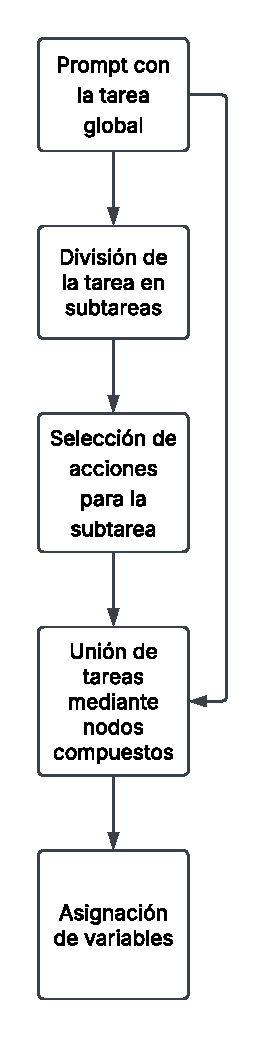
\includegraphics[width=0.2\textwidth]{Imagenes/Vectorial/GeneracionSubtareas.pdf}
    \caption[Generación mediante subtareas]{Diagrama de flujo de la generación de \glspl{BT} mediante división en subtareas}
    \label{fig:generacionSubtareas}
\end{figure}

Finalmente se descartó esta opción debido a que los árboles resultantes quedaban muy planos (con menos niveles de profundidad de lo que se cabía esperar), hacieéndolos difícilmente legibles y modificables.
Además los agentes tendían a equivocarse (mala división en subtareas, confusión entre el tipo que debería ser un nodo padre) o a alucinar (inventarse tareas o decoradores que no existen), no consiguiendo de este modo un \gls{BT} válido con ninguno de los modelos probados.

Trabajos como \cite{SayCan} o \cite{LLMPlanner} muestran que, dado un conjunto de acciones posibles a realizar, los \glspl{LLM} son capaces de seleccionar de éstas un órden para realizar una tarea de alto nivel.
Es por ésto que se decidió que el \gls{LLM} generase esta secuencia en un formato de pseudocódigo que fuese fácilmente convertible al formato JSON deseado.
Este pseudocódigo se especifica de la siguiente manera:
\begin{itemize}
    \item Las palabras reservadas son: SEQUENCE, SELECTOR, PARALLEL, IF, THEN, ELSE, DO, END.
    \item Los bloques de nodos compuestos (como SELECTOR) deben acabar con la palabra END.
    \item Las condiciones deberán ser escritas como ``IF (nombre del condicional de la lista de decoradores) THEN''.
    \item Los condicionales serán usados por el nodo siguiente.
    \item Las acciones deberán ser escritas como ``DO (nombre de la acción de la lista de acciones)''. 
\end{itemize}

Se puede ver un ejemplo de este pseudocódgo en la figura \ref{fig:examplePseudocode}.

\begin{figure}[htbp]
  \begin{verbatim}
SELECTOR
    IF has_key THEN
        SEQUENCE
            DO move_to_door
            DO open_door
        END
    ELSE
        SEQUENCE
            DO find_key
            DO move_to_door
            DO open_door
        END
END
\end{verbatim}
  \caption{Ejemplo del pseudocódigo que el \gls{LLM} debe generar.}
  \label{fig:examplePseudocode}
\end{figure}

Como se ha podido ver en trabajos relacionados, la generación de \glspl{BT} mediante \glspl{LLM} mejora considerablemente en modelos a los que se le ha aplicado \gls{Fine-tuning} o se les proporciona ejemplos.
Debido a la falta de capacidad computacional no se ha podido hacer un \gls{Fine-tuning} de un \gls{LLM}, por lo que se ha optado a recopilar una pila de ejemplos de \glspl{BT} para poder hacer un sistema \gls{RAG}.
Para ello se ha escogido el dataset publicado por \cite{llmbrain}\footnote{Enlace a la página de Hugging Face: \url{https://huggingface.co/datasets/ArtemLykov/LLM_BRAIn_dataset}}, el cual contiene 8366 ejemplos de \glspl{BT}.
Debido a que estos \glspl{BT} están en formato XML no se pueden utilizar de forma predeterminada para el sistema RAG, por lo que se ha procedido a hacer un preprocesamiento de los datos.
Este proprocesado carga el dataset desde Hugging Face, los limpia y los traduce al formato necesario.
La limpieza consiste en el uso de expresiones regulares para poder subsanar los fallos de formato más comunes que tenían estos datos, como diferencias entre nombres por mayúsculas y minúsculas, etiquetas sin la apertura o la clausura, faltas de comillas, etc.
Si hay algún ejemplo que, aun con la limpieza, no se ha conseguido parsear por otro fallo, se descarta.
Finalmente, de los 8366 ejemplos se quedaron 8290 \glspl{BT} válidos.
Una vez los datos están limpios, se procede a la traducción del formato XML gracias al módulo ``xml.etree.ElementTree'' mediante una función recursiva que recorre el XML y va construyendo todo el árbol.
Cuando el árbol ha sido construído se guarda en formato JSON siguiendo el JSON Schema especificado para este trabajo, y finalmente se traduce al pseudocódigo especificado previamente gracias a otra función recursiva, quedando así 8366 archivos JSON con el prompt de la acción de alto nivel a realizar, el \gls{BT} resultante y el pseudocódigo.

Con los ejemplos de \glspl{BT} preparados se ha procedido a la aplicación del sistema \gls{RAG}.
Al iniciar la herramienta de generación se crea el \gls{Almacén vectorial} cargando los documentos mencionados anteriormente en estructuras llamadas ``Document'', provenientes del módulo ``langchain\_core.documents''.
Una vez están todos los documentos cargados se procede a hacer el \gls{Embedding} de éstos de manera local gracias al modelo de Hugging Face ``all-MiniLM-L6-v2'' mediante el módulo ``langchain\_huggingface''.
Estos \glspl{Embedding} se crean y se almacenan en una estructura de tipo \gls{FAISS} gracias al módulo ``langchain\_community.vectorstores''.
Una vez creado el \gls{Almacén vectorial} se rescatan las 5 búsquedas más similares al comportamiento pedido por el usuario y se incluyen en el prompt del sistema del \gls{LLM}.

Para la generación de pseudocódgo a partir del comportamiento buscado se ha requerido un modelo de mayor tamaño que los previamente usados, por lo que se ha usado el \gls{LLM} ``Mistral Large 3'', el cual cuenta con un total de 41B de parámetros, mediante el módulo ``langchain\_mistralai'', el cual realiza llamadas de \gls{api} al modelo.
Para el prompt de sistema del modelo se han realizado varias técnicas de \textit{prompt engineering} con el fin de reducir las alucinaciones en la generación del pseudocódgo:

\begin{itemize}
    \item \texttt{Role prompting}: Se le especifica al \gls{LLM} como debe actuar: ``You are an expert in behavior trees and algorithm design.''.
    \item \texttt{Especificación de la tarea}: Se le especifica para qué tarea debe responder: ``Your task is to convert a high-level task description into a structured pseudocode algorithm that can later be transformed into a Behavior Tree.''.
    \item \texttt{Few-shot prompting}: Se le especifican varios ejemplos, sacados del sistema \gls{RAG} mencionado anteriormente.
    \item \texttt{Chain-of-Thought}: Obliga al modelo a, internamente, seguir la línea de pensamiento representada en la figura \ref{fig:CoT-Code}
    \item \texttt{Self‑Critique Prompting}: Le pide al modelo que evalúe su respuesta buscando si se ha inventado acciones o condicionales. Esto se hace en una segunda llamada con el siguiente prompt: ``Verify if your pseudocode is made only with the actions and conditions available. Responde me with ONLY the final pseudocode and no explanations or plain text''
\end{itemize}

\begin{figure}[H]
    \centering
    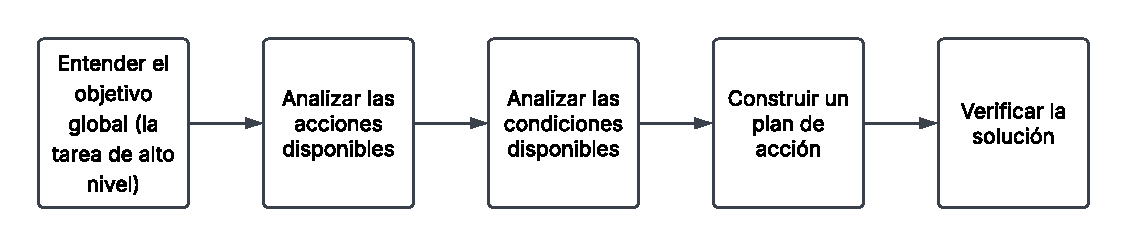
\includegraphics[width=1\textwidth]{Imagenes/Vectorial/CoT-TFM.pdf}
    \caption[Chain-of-Thought del \gls{LLM} que genera el pseudocódgo.]{Diagrama de la cadena de pensamiento que sigue el \gls{LLM} generador de pseudocódigo.}
    \label{fig:CoT-Code}
\end{figure}

El prompt de sistema completo se puede ver en el apéndice \ref{appendix:spCode}.

Una vez se ha generado el pseudocódigo se procede a la traducción de éste al formato JSON.
Esto se hace mediante la clase ``BehaviorTreeParser'' y mediante dos clases auxiliares: Composite y Action, las cuales ambas heredan de la clase Node.
La clase Composite contiene el tipo (un string), una lista de nodos hijos (lista de tipo ``Node''), un decorador (opcional de tipo string), las variables de la \gls{BB} del decorador (una lista de strings) y un identificador (un entero).
La clase Action tiene el nombre de la tarea (un string), las variables de la \gls{BB} que puede usar la tarea (una lista de strings), un decorador (opcional de tipo string), las variables de la \gls{BB} del decorador (una lista de strings) y un identificador (un entero).
Para la traducción del pseudocódigo primero se preprocesa guardando cada línea en una lista de strings.
Seguido de esto se procesa cada línea dividiendo cada palabra de ésta y actuando dependiendo de cuál es su primera palabra:
\begin{itemize}
    \item \texttt{SEQUENCE, SELECTOR o PARALLEL}: Se crea un nodo de tipo ``Composite'', se establece su tipo como la palabra usada y se verifica si hay una condición pendiente. Si es el caso, se establece esta condición. Además, se añade este nodo a su padre (en el caso de haberlo es el último nodo añadido a una pila auxiliar) y se añade a la pila auxiliar.
    \item \texttt{IF}: Se verifica si tiene un condicional o si el condicional que tiene existe. En caso contrario de cualquiera de los dos se lanza un ``ParserError'' indicando la línea y el fallo. En el caso de que no haya error se establece la condición como la condición pendiente.
    \item \texttt{DO}: Se verifica si tiene una acción o si esa acción existe. Al igual que en el caso anterior, de no ser así se lanza un ``ParserError''. En caso de haberlo se crea un nodo de tipo ``Action'' con el nombre de la acción que hay a continuación. Igualmente que con los nodos compuestos, se verifica si hay alguna condición pendiente y se añade el nodo al padre.
    \item \texttt{END}: Se verifica que la pila no esté vacía. En caso contrario significa que hay un ``END'' sin bloque que cierre, por lo que se lanza un ``ParserError''. En caso de que sí esté vacía se saca un nodo de la pila. A continuación se verifica si la pila se ha quedado vacía, lo que significaría que ese nodo era la raíz del árbol. En caso de ya haber raíz se lanza un ``ParserError'' indicando que hay múltiples raíces.
\end{itemize}
Una vez se acaba este procesamiento de cada línea se verifica si sigue habiendo pila (lo que indicaría que hay bloques sin cerrar) o si no se ha generado una raíz.
Los posibles ``ParserError'' lanzados durante este proceso se recogen fuera de esta función para poder volver llamar al \gls{LLM} indicando el error de la excepción con el fin de que devuelva un pseudocódigo arreglado.

Cuando ya ha sido procesado todo el pseudocódigo se crea una clase auxiliar llamada ``BlackboardAssignmentAgent'' que se encarga de asignar las variables de la \gls{BB} a las tareas o los decoradores.
Para ello reconstruye el pseudocódigo asignándole el identificador a cada nodo (este identificador es el órden de aparición de cada acción o decorador, ya que en los \glspl{BT} es normal que se repitan) y se le pide a un segundo \gls{LLM} que a cada decorador y acción que necesite una variable de la \gls{BB} se le asigne.
Por problemas con sobrecarga de peticiones de la \gls{api}, para este caso se usa un modelo local más pequeño, el modelo ``llama3:8b''.
Para el prompt de sistema de este \gls{LLM} se le pasa el árbol en el formato del pseudocódigo reconstruido mencionado anteriormente, la lista de las acciones que necesitan una variable de la \gls{BB} con sus descripciones y la lista de variables de la \gls{BB}.
Para disminuir las alucinaciones de este \gls{LLM} se han usado las siguientes técnicas de \textit{prompt engineering}:

\begin{itemize}
    \item \texttt{Role prompting}: ``You are an expert in Unreal Engine Behavior Trees.''
    \item \texttt{Especificación de la tarea}: ``Your task is NOT to understand the whole game. Your ONLY task is assigning Blackboard variables to Behavior Tree nodes.''
    \item \texttt{One-shot prompting}: Se le especifica un ejemplo inventado mostrado en la figura \ref{fig:examplePseudocodeBB}
\end{itemize}

\begin{figure}[htbp]
  \begin{verbatim}
Example Input:
Actions : grab_key : Stores the key in the inventory,
    move_to : Moves to a position,
    open_door: Open a door
Variables: ["Key" : "Object", "Door" : "Object", "Enemy_position" : "Vector3"]
Tree:
SEQUENCE
    DO move_to#1
    DO grab_key#1
    DO move_to#2
    DO open_door#1 [Decorator=IsNear?#1]
    DO wave#1

Output format: 
{
    "Actions": {
        "move_to#1":["Key"],
        "grab_key#1":["Key"],
        "move_to#2":["Door"],
        "open_door#1":["Door"]
    },

    "Decorators": {
        "IsNear?#1":["Door"]
    }
}
\end{verbatim}
  \caption{Ejemplo del input y el output del \gls{LLM} que establece las variables de la \gls{BB}.}
  \label{fig:examplePseudocodeBB}
\end{figure}

Una vez genera la respuesta se valida el resultado comprobando si todos los nombres (variables y acciones) son correctos.
Cuando el resultado es válido se guardan las variables asignadas en los nodos correspondientes y, finalmente, se construye el JSON mediante una función recursiva desde la raiz del árbol y se guarda en un archivo con el nombre especificado por el usuario.

Trabajos como \cite{PlanBench} han demostrado que la planificación generada por \glspl{LLM} como se ha hecho en este trabajo no resultan ser fiables de forma exacta, por lo que se ha diseñado un sistema de validación y corrección de errores automático.
\section{Validación automática de los \glspl{BT}}
\label{sec:Validacion}

Para que los \glspl{BT} generados se considerasen válidos para las pruebas se han tenido en cuenta dos factores: que los árboles generados respeten el órden de los nodos (si hay acciones dependientes unas con otras no deben ejecutarse los hijos antes que los padres) y que deben cumplir un objetivo.
Estas comprobaciones no son obligatorias para el funcionamiento de la herramienta, sino que es un apoyo para automatizar este proceso.

\subsection{Validación de dependencias}
Para comprobar el órden correcto de los nodos se ha recurrido al uso de un autómata finito no determinista, NFA por las siglas en inglés de Non-Deterministic Finite Automata (\cite{NFA}, \cite{NFAPlan}), definido de la siguiente manera:
\begin{itemize}
    \item Los estados son los nodos de \gls{BT}.
    \item Las transiciones son las relaciones padre-hijo.
    \item El alfabeto son las IDs de las tareas.
    \item Hay un conjunto de estados abiertos.
    \item Hay una serie de estados iniciales.
    \item La función de transición es no determinista porque un mismo símbolo puede activar múltiples nodos de forma simultánea, ya que diferentes tareas pueden estar en diferentes puntos del árbol.
\end{itemize}
Este NFA está implementado en la clase ``BehaviorList'', la cual está implementada mediante el patrón Singleton para que todas las tareas puedan acceder a ella.
Para esta verificación se necesita un archivo JSON en el que se especifican las restricciones.
Se puede ver un ejemplo de un JSON con las restricciones en el apéndice \ref{appendix:Orden}.

Una vez se construyan las dependencias mediante el NFA empieza la ejecución del BT.
Para que funcione esta comprobación a la hora de ejecutarse una tarea o un decorador, éste debe llamar a la función ``addBehavior'' de esta clase con el nombre de la tarea.
Cuando llega una tarea nueva se realiza la comprobación de las dependencias de la siguiente forma:

\begin{enumerate}
    \item Se recuperan los nodos candidatos gracias a su ID.
    \item Se crea un nuevo conjunto de nuevos estados.
    \item Si un candidato no tiene padre (no depende de ninguna otra acción) se añade este nodo a los nuevos posibles estados.
    \item Se recorren todos los hijos de los estados activos y se comprueba si coinciden con el ID de la tarea o el decorador actual. En caso afirmativo se añade este hijo al conjunto de nuevos estados.
\end{enumerate}

Al final de la función se comprueba si el conjunto de nuevos estados está vacío.
En el caso de que el conjunto de nuevos estados no está vacío implica que sí se han respetado las dependencias, por lo que éste pasa a ser el conjunto de estados abiertos.
Por el otro lado, si el conjunto de nuevos estados está vacío es que no existe ningún posible estado en el que el órden de la ejecución de los nodos sea la actual, lo que implica que no se han respetado las dependencias y la validación falla.

Para los casos en los que la validación puede fallar se ha creado una clase interfaz ``IValidatorCallback'' que se encarga de gestionar las terminaciones de la validación por fallos o por terminación de la ejecución.
Ya que es la clase ``GeneratorComponent'' quien se encarga de llamar a la herramienta de generación, es esta quien hereda de la interfaz y quien es llamada por la clase ``BehaviorList'' cuando falla la validación, pasándole una lista de todas las acciones ejecutadas hasta el momento y la acción en la que ha fallado.
Es entonces cuando la clase ``GeneratorComponent'' interrumpe el modo de juego y vuelve a llamar a la herramienta con el pseudocódigo fallido, el contexto dado por ``BehaviorList'' y el prompt con la acción original y vuelve a intentar la ejecución cuando la herramienta arregla el psuedocódigo.

\subsection{Validación de objetivos}
Para validar los objetivos específicos de los comportamientos se ha creado una clase interfaz ``ObjectiveValidatorBase'' que contiene un método para comprobar si el objetivo se ha cumplido y un mensaje de error indicando que el objetivo ha fallado.
De esta interfaz deben heredar componentes de Actor para que los objetos ``BTGeneratorManager'' los puedan tener y puedan hacer la comprobación de los objetivos una vez se acabe la ejecución.
Si la comprobación del objetivo es fallida se le pasa a la herramienta el mensaje de error y la lista de tareas ejecutadas, así como el pseudocódigo fallido y el prompt original, y se vuelve a intentar con un pseudocódigo arreglado.

\subsection{Entornos creados para la validación}
Una vez se han tenido los métodos de validación de los BTs se han creado tres entornos con diferentes pruebas.

El primero de ellos consta de tres flores de distintos colores: rojo, azul y amarillo.
En este entorno se le pide a la herramienta que genere un BT donde recoja una única flor de cada tipo, independientemente del órden, con el siguiente prompt: ``NPC that has to choose and pick one flower red, one flower yellow, and one flower blue. In order to pick a flower it has to be first in the position of the flower.''.
Al ser una tarea sencilla la herramienta solo ha necesitado un intento y un tiempo de ejecución de 84.84 segundos para crear un BT válido y que cumpla con el objetivo.

El segundo de los entornos consta de tres flores azules, una flor roja y una flor amarilla, y aquí se le pide a la herramienta que genere un BT que recoja tres flores azules y después una roja mediante el siguiente prompt: ``NPC that has to choose and then pick first three blue flowers, and, after that, has to choose and pick one red flower. In order to pick a flower it has to be first in the position of the flower''.
Al igual que en el caso anterior, solo ha necesitado de un intento y un tiempo de 45.46 segundos para realizar un BT válido.
En la figura \ref{fig:escenario2} se puede ver una captura de pantalla de este entorno.

\begin{figure}[H]
    \centering
    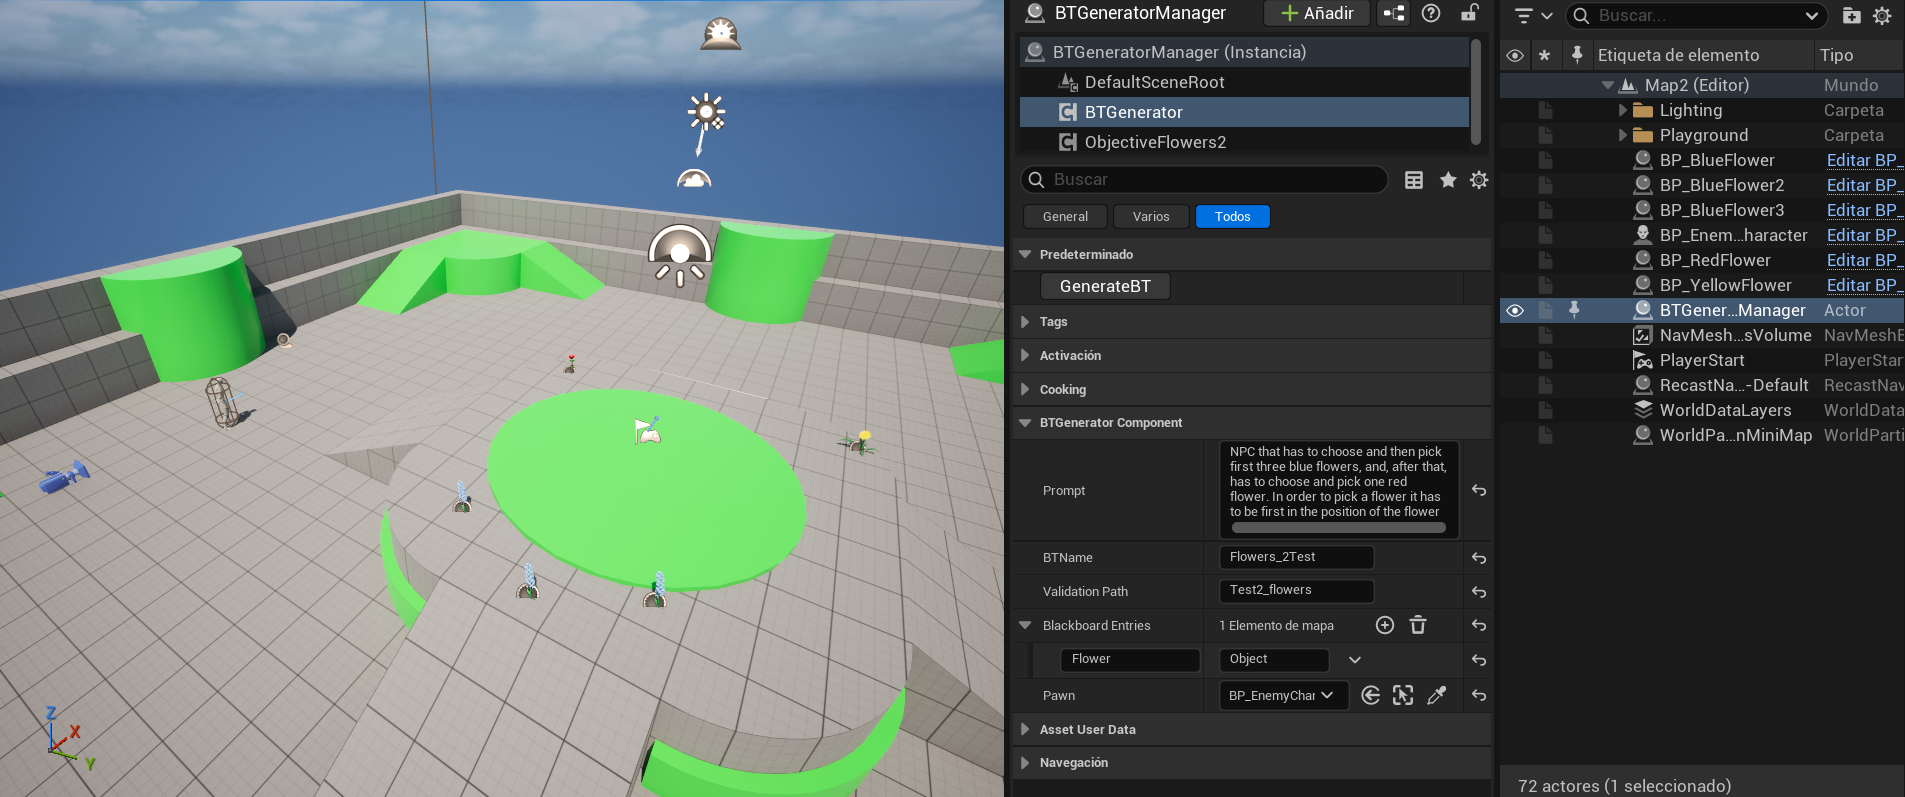
\includegraphics[width=1\textwidth]{Imagenes/Bitmap/Entorno2.png}
    \caption[Captura de pantalla del segundo entorno]{Captura de pantalla del segundo entorno de pruebas de validación.}
    \label{fig:escenario2}
\end{figure}

El tercer entorno consta de un enemigo y un punto de patrulla.
Aquí se le pide a la herramienta que genere un comportamiento clásico en videojuegos: un NPC que patruye el escenario por distintos puntos y, que si ve al jugador, le persiga para atacarle.
Para ello se ha usado el siguiente prompt: ``NPC that has to do one of this two options:
- If the objective is at his line of sight it has to: 1. chase him 2. move to his position 3. if is near the objective, it has to attack him.
- Otherwise, it has to: 1. select a waypoint 2. move to the waypoint''.

A pesar de ser una petición más compleja debido a la naturaleza del comportamiento y al aumento de número de variables de la Blackboard (cuatro variables, dos condicionales para ver si el objetivo está en el punto de mira y si el objetivo está cerca, el punto de patrulla a elegir y el objetivo a perseguir), la herramienta ha sido capaz de generar en 153.1 segundos un BT válido a la primera en cuanto a cumplimiento de objetivos y respetando las dependencias, aunque sí se ha tenido que modificar alguna tarea que requería de una variable de la Blackboard que el segundo LLM no le ha adjudicado ninguna variable.
En la figura \ref{fig:escenario3} se puede ver una captura de pantalla de este tercer entorno.

\begin{figure}[H]
    \centering
    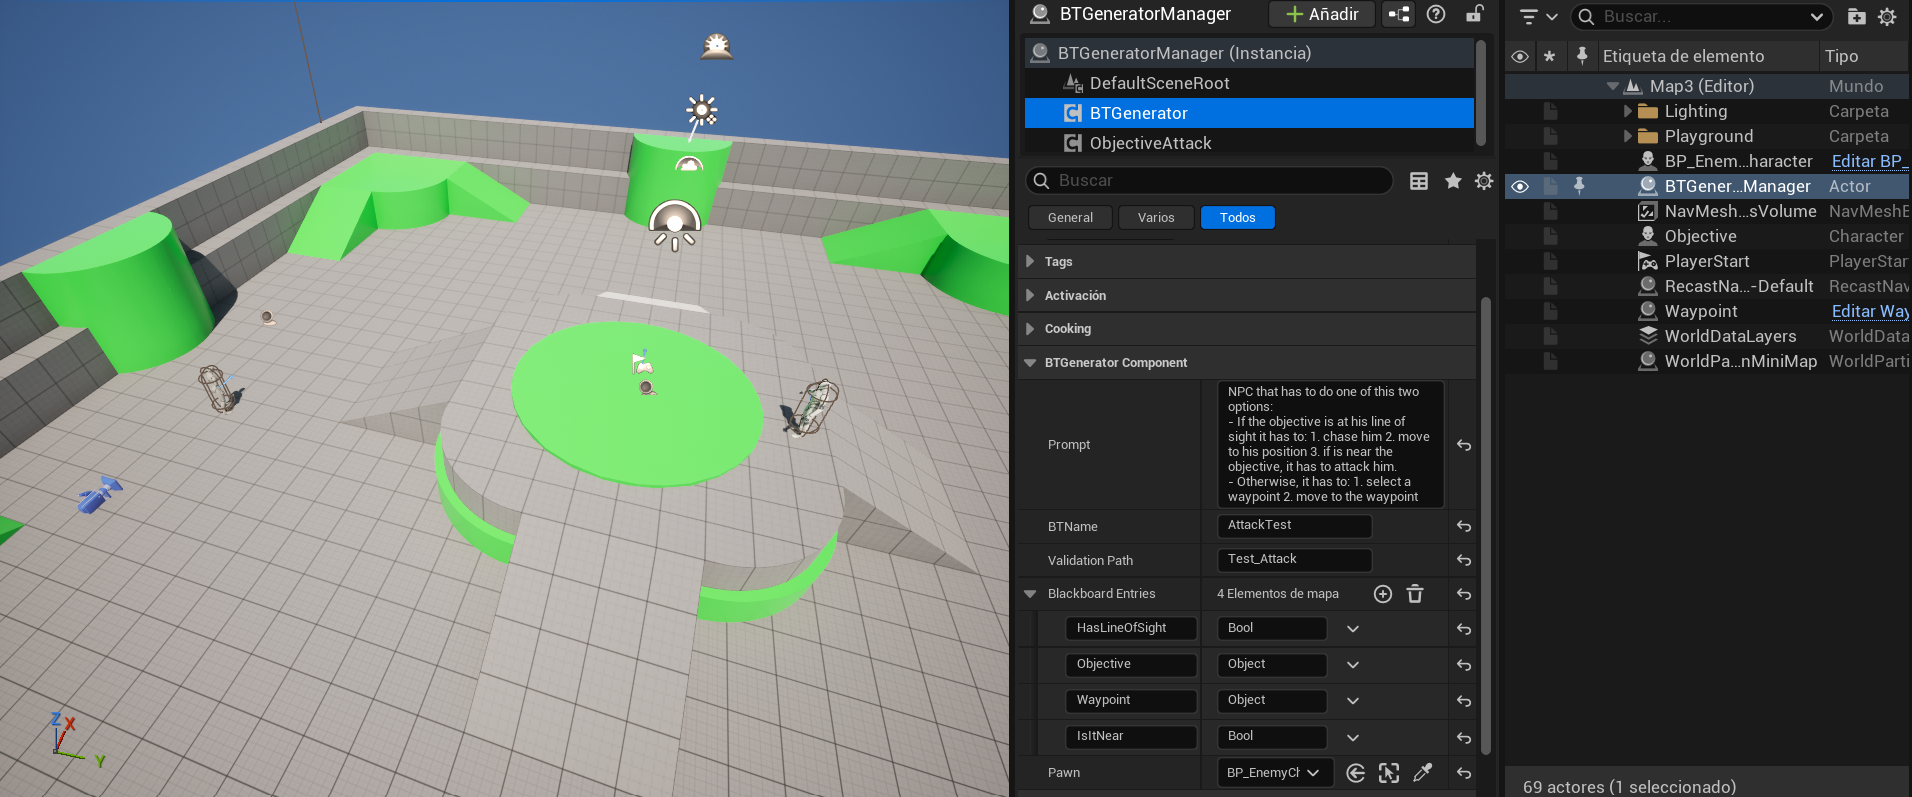
\includegraphics[width=1\textwidth]{Imagenes/Bitmap/Entorno3.png}
    \caption[Captura de pantalla del tercer entorno]{Captura de pantalla del tercer entorno de pruebas de validación.}
    \label{fig:escenario3}
\end{figure}

Con los resultados de esta validación, resumidos en la tabla \ref{tab:validacion}, se ha podido establecer un baseline del funcionamiento de la herramienta para, finalmente, realizar pruebas con usuarios.

\begin{longtblr}[
    caption = {Resultados de las pruebas de validación},
    label = {tab:validacion}
]{
colspec={|l|l|l|},
rowhead=1,
hlines,
row{even}={gray9},
cells   = {font=\footnotesize\linespread{0.84}\selectfont},
}
    \hline
    Entorno    & Intentos  & Tiempo de ejecución\\ \hline
    1    & 1   & 84.84 segundos \\
    2    & 1  & 45.46 segundos \\
    3  & 1  &  153.1 segundos \\ \hline
\end{longtblr}
